% Provenance (never printed): cycle 3 geography and "La planete Terre"
% (the great physical features of the world: relief, rivers, deserts, ice;
% reading a physical map); see sources/book1/PROVENANCE.md.
% Book 1, grade 4, chapter 3.
\chapter{الخريطة الطبيعية للعالم}\label{ch:g4:world-physical-map}

يفرد سامي ونور \omterm{def:g2:drawing-to-map:map}{خريطة} كبيرة للعالم على أرض الفصل ويجثوان حولها. إنها لا
تشبه الخرائط التي يعرفانها. فلا بلدان فيها، ولا حدود، ولا مدن. بل اليابسة
ملوّنة: أخضر على \omterm{def:g1:landscapes-around-us:water}{السواحل} وفي الأراضي المنبسطة الواسعة، ثم أصفر فاتح، ثم
بني، وفي أماكن قليلة أبيض تقريبًا. \omterm{def:g2:water-on-earth:ocean}{والبحر} أيضًا له درجات من الأزرق: فاتح
قرب \omterm{def:g1:landscapes-around-us:water}{السواحل}، ثم أدكن فأدكن كلما ابتعدنا في عرض
المحيطات.

تسأل نور: «لماذا هذا الجزء من آسيا أبيض؟ أهو \omterm{def:g4:clouds-rain-snow:precipitation}{ثلج}؟» ليس تمامًا. ففي هذه
\omterm{def:g2:drawing-to-map:map}{الخريطة}، كل لون يخبرنا كم ترتفع اليابسة، أو كم يعمق \omterm{def:g2:water-on-earth:ocean}{البحر}.

\begin{recall}
\omterm{def:g2:drawing-to-map:map}{الخريطة} تبين مكانًا من الأعلى، مصغرًا؛ \omterm{def:g2:drawing-to-map:legend}{ومفتاحها} يشرح ألوانها ورموزها
(\cref{ch:g2:drawing-to-map}). واليابسة مجموعة في سبع \omterm{def:g3:continents-and-oceans:continent}{قارات}، بين خمسة
محيطات، \omterm{def:g3:continents-and-oceans:world-map}{وخريطة العالم} \omterm{def:g3:continents-and-oceans:globe}{مجسم كرة أرضية} مبسوط
(\cref{ch:g3:continents-and-oceans}). \omterm{def:g1:landscapes-around-us:landform}{والجبال} \omterm{def:g1:landscapes-around-us:landform}{والتلال} \omterm{def:g1:landscapes-around-us:landform}{والوديان} \omterm{def:g1:landscapes-around-us:landform}{والسهول} هي
\omterm{def:g1:landscapes-around-us:landform}{الأشكال التضاريسية}؛ \omterm{def:g1:landscapes-around-us:water}{والأنهار} تجري من الأرض المرتفعة نزولًا إلى \omterm{def:g2:water-on-earth:ocean}{البحر}
(\cref{ch:g1:landscapes-around-us}).
\end{recall}

\section{قراءة الخريطة الطبيعية}

لكي نقول كم يرتفع مكان ما، نحتاج إلى مستوى ننطلق منه، هو نفسه في كل مكان
على الأرض. فنأخذ \omterm{def:g4:world-physical-map:altitude}{مستوى سطح البحر}.

\begin{definition}[الارتفاع ومستوى سطح البحر]\label{def:g4:world-physical-map:altitude}
\emph{مستوى سطح البحر}\index{مستوى سطح البحر} هو المستوى المتوسط لسطح
\omterm{def:g2:water-on-earth:ocean}{البحر}، بين المد والجزر. و\emph{الارتفاع}\index{ارتفاع} لمكان ما هو علوّه
فوق مستوى سطح \omterm{def:g2:water-on-earth:ocean}{البحر}، بالأمتار. وتحت \omterm{def:g2:water-on-earth:ocean}{البحر} نتحدث عن \emph{العمق}: أي كم
يقع قاع \omterm{def:g2:water-on-earth:ocean}{البحر} تحت مستوى سطح \omterm{def:g2:water-on-earth:ocean}{البحر}.
\end{definition}

بلدة على شاطئ \omterm{def:g2:water-on-earth:ocean}{البحر} ارتفاعها بضعة أمتار. أما قرية في \omterm{def:g1:landscapes-around-us:landform}{الجبال} فقد تقع على
\omterm{def:g4:world-physical-map:altitude}{ارتفاع} 1\,500 متر: أي كيلومتر ونصف فوق \omterm{def:g4:world-physical-map:altitude}{مستوى سطح البحر}، حتى لو كانت على
بعد مئات الكيلومترات من أي \omterm{def:g1:landscapes-around-us:water}{ساحل}.

\begin{definition}[التضاريس]\label{def:g4:world-physical-map:relief}
\emph{التضاريس}\index{تضاريس} لمنطقة ما هي شكل أرضها: أين ترتفع وأين
تنخفض، وجبالها وهضابها ووديانها
وسهولها.
\end{definition}

\begin{definition}[الخريطة الطبيعية]\label{def:g4:world-physical-map:physical-map}
\emph{الخريطة الطبيعية}\index{خريطة طبيعية} تبين \omterm{def:g4:world-physical-map:relief}{تضاريس} اليابسة وعمق
\omterm{def:g2:water-on-earth:ocean}{البحر} بالألوان، لونًا لكل درجة من \omterm{def:g4:world-physical-map:altitude}{الارتفاع} أو العمق، وتبين \omterm{def:g1:landscapes-around-us:water}{الأنهار}
الكبرى \omterm{def:g1:landscapes-around-us:water}{والبحيرات} والصحاري والجليد.
\end{definition}

\begin{omfigure}
\begin{tikzpicture}
\begin{axis}[ommap, width=\linewidth, xtick=\empty, ytick=\empty, grid=none,
    axis background/.style={}, clip=true]
  \addplot graphics[xmin=-180, xmax=180, ymin=-90, ymax=90]
    {figdata/out/grade-4-physical_map.png};
  \addplot[black!45, line width=0.15pt] table {figdata/out/shared-geo-land.dat};
  \addplot[fill=omHypsSeaB, draw=blue!60!black, line width=0.2pt]
    table {figdata/out/grade-4-physical_map-lakes.dat};
  \addplot[blue!70!black, line width=0.5pt] table {figdata/out/grade-4-physical_map-rivers.dat};
  \begin{scope}[every node/.style={font=\scriptsize\bfseries, align=center,
      fill=white, fill opacity=0.7, text opacity=1, inner sep=1pt, rounded corners=1pt}]
    \node at (axis cs:-112,47) {جبال\\روكي};
    \node at (axis cs:-62,-22) {الأنديز};
    \node at (axis cs:10,49) {الألب};
    \node at (axis cs:84,24) {الهيمالايا};
    \node at (axis cs:4,23) {الصحراء الكبرى};
    \node at (axis cs:-40,74) {غرينلاند\\\foreignlanguage{arabic}{(جليد)}};
    \node at (axis cs:60,-80) {جليد القارة القطبية الجنوبية};
  \end{scope}
  \begin{scope}[every node/.style={font=\scriptsize\itshape, text=blue!50!black,
      fill=white, fill opacity=0.6, text opacity=1, inner sep=1pt}]
    \node at (axis cs:38,17) {النيل};
    \node at (axis cs:-56,-7) {الأمازون};
    \node at (axis cs:-80,33) {المسيسيبي};
    \node at (axis cs:118,26) {اليانغتسي};
  \end{scope}
\end{axis}
\end{tikzpicture}

\smallskip
\begin{tikzpicture}[font=\scriptsize, x=1.18cm]
  \foreach \i/\c/\t in {0/5A9CCF/{أعمق من\\\babelsublr{4000}}, 1/84BCE0/{\foreignlanguage{arabic}{من \babelsublr{2000}}\\\foreignlanguage{arabic}{إلى \babelsublr{4000}}},
      2/B3D8EE/{\foreignlanguage{arabic}{من \babelsublr{200}}\\\foreignlanguage{arabic}{إلى \babelsublr{2000}}}, 3/DCEEF8/{\foreignlanguage{arabic}{من \babelsublr{0}}\\\foreignlanguage{arabic}{إلى \babelsublr{200}}}} {
    \definecolor{tmp}{HTML}{\c}
    \fill[tmp, draw=black!40] (\i,0) rectangle (\i+0.92,0.35);
    \node[align=center, anchor=north] at (\i+0.45,-0.05) {\t};
  }
  \foreach \i/\c/\t in {5/9CC98A/{\foreignlanguage{arabic}{من \babelsublr{0}}\\\foreignlanguage{arabic}{إلى \babelsublr{200}}}, 6/C9DE99/{\foreignlanguage{arabic}{من \babelsublr{200}}\\\foreignlanguage{arabic}{إلى \babelsublr{500}}},
      7/F1E7A8/{\foreignlanguage{arabic}{من \babelsublr{500}}\\\foreignlanguage{arabic}{إلى \babelsublr{1000}}}, 8/E5C58A/{\foreignlanguage{arabic}{من \babelsublr{1000}}\\\foreignlanguage{arabic}{إلى \babelsublr{2000}}}, 9/C79E76/{\foreignlanguage{arabic}{من \babelsublr{2000}}\\\foreignlanguage{arabic}{إلى \babelsublr{4000}}},
      10/ECE8E3/{أعلى من\\\babelsublr{4000}}} {
    \definecolor{tmp}{HTML}{\c}
    \fill[tmp, draw=black!40] (\i,0) rectangle (\i+0.92,0.35);
    \node[align=center, anchor=north] at (\i+0.45,-0.05) {\t};
  }
  \node[anchor=south] at (2,0.4) {\foreignlanguage{arabic}{عمق البحر \babelsublr{(m)}}};
  \node[anchor=south] at (8,0.4) {\foreignlanguage{arabic}{ارتفاع اليابسة \babelsublr{(m)}}};
\end{tikzpicture}

{\small \omterm{def:g4:world-physical-map:physical-map}{الخريطة الطبيعية} للعالم، مع \omterm{def:g2:drawing-to-map:legend}{مفتاحها}. كل لون درجة من \omterm{def:g4:world-physical-map:altitude}{الارتفاع} (على
اليابسة) أو من العمق (تحت \omterm{def:g2:water-on-earth:ocean}{البحر}). \omterm{def:g1:landscapes-around-us:water}{والأنهار} باللون الأزرق الداكن. وقد رُسمت
\omterm{def:g4:world-physical-map:relief}{التضاريس} من قيمة واحدة لكل درجة من درجات العرض والطول (أي نحو كل 100
كيلومتر)، فهي ملساء: فلا تظهر القمم المنفردة ولا الأغوار الضيقة. البيانات:
تضاريس ETOPO1 من NOAA؛ \omterm{def:g1:landscapes-around-us:water}{الأنهار} \omterm{def:g1:landscapes-around-us:water}{والبحيرات} \omterm{def:g1:landscapes-around-us:water}{والسواحل} من
Natural Earth.}
\label{fig:g4:world-physical-map:map}
% ledger: data:etopo1, data:b1-ne-rivers, data:ne-land
\end{omfigure}

\begin{method}[قراءة لون على الخريطة الطبيعية]\label{met:g4:world-physical-map:reading}
لتجد \omterm{def:g4:world-physical-map:altitude}{ارتفاع} مكان على \omterm{def:g4:world-physical-map:physical-map}{خريطة طبيعية}:
\begin{enumerate}
  \item جد المكان، وانظر إلى لونه؛
  \item جد اللون نفسه في \omterm{def:g2:drawing-to-map:legend}{المفتاح}؛
  \item اقرأ الدرجة تحته: \omterm{def:g4:world-physical-map:altitude}{ارتفاع} المكان يقع بين
        العددين.
\end{enumerate}
والطريقة نفسها تصلح في \omterm{def:g2:water-on-earth:ocean}{البحر}، للعمق.
\end{method}

\begin{example}[ثلاثة أماكن]\label{ex:g4:world-physical-map:three}
مصب الأمازون، على \omterm{def:g1:landscapes-around-us:water}{ساحل} أمريكا الجنوبية، أخضر داكن: ارتفاعه بين 0 و200
متر. ووسط الصحراء الكبرى أخضر فاتح أو أصفر فاتح: بين 200 و1\,000 متر.
والهضبة الواقعة شمال الهيمالايا، في آسيا، بيضاء تقريبًا: فوق 4\,000
متر.
\end{example}

\section{السلاسل الجبلية الكبرى}

على \omterm{def:g2:drawing-to-map:map}{الخريطة}، لا ينتشر اللونان البني والأبيض انتشارًا منتظمًا. بل يصنعان
أشرطة طويلة ضيقة.

\begin{definition}[السلسلة الجبلية]\label{def:g4:world-physical-map:range}
\emph{السلسلة الجبلية}\index{سلسلة جبلية} صف طويل من \omterm{def:g1:landscapes-around-us:landform}{الجبال} المتصلة بعضها
ببعض، يمتد مئات الكيلومترات أو آلافها.
\end{definition}

تمتد \omterm{def:g1:landscapes-around-us:landform}{جبال} الأنديز على طول الجانب الغربي كله لأمريكا الجنوبية. ولأمريكا
الشمالية \omterm{def:g1:landscapes-around-us:landform}{جبال} روكي، ولأوروبا \omterm{def:g1:landscapes-around-us:landform}{جبال} الألب، ولآسيا أعلاها جميعًا: \omterm{def:g1:landscapes-around-us:landform}{جبال}
الهيمالايا. وهناك يقوم أعلى \omterm{def:g1:landscapes-around-us:landform}{جبل} على الأرض: \omterm{def:g1:landscapes-around-us:landform}{جبل} إفرست، وارتفاعه
8\,849 مترًا، بحسب قياس جديد أُجري عام 2020.
% ledger: tht:everest

\begin{omfigure}
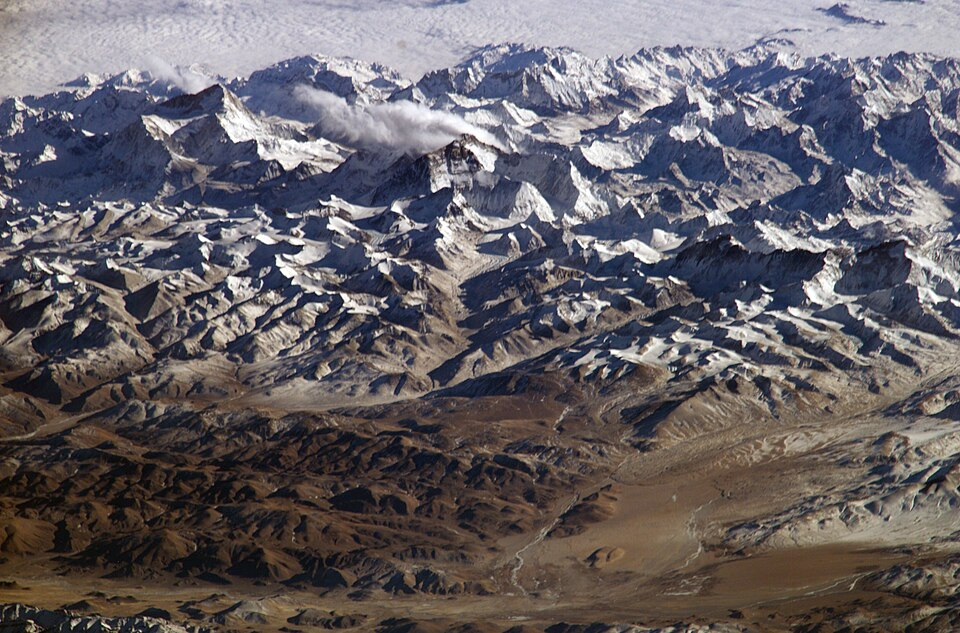
\includegraphics[width=0.75\linewidth]{images/book1/g4-himalaya-iss.jpg}

{\small \omterm{def:g1:landscapes-around-us:landform}{جبال} الهيمالايا كما تُرى من محطة الفضاء الدولية، والنظر متجه
جنوبًا من هضبة التبت العالية: \omterm{def:g2:water-on-earth:ocean}{بحر} من القمم المكسوة \omterm{def:g4:clouds-rain-snow:precipitation}{بالثلج}.
الصورة: NASA (ملك عام).}
% ledger: nasa:himalaya-iss
\end{omfigure}

\section{الأنهار والبحيرات الكبرى}

\omterm{def:g4:clouds-rain-snow:precipitation}{المطر} \omterm{def:g4:clouds-rain-snow:precipitation}{والثلج} الذائب يجريان على الأرض، فيجتمعان في جداول ثم في \omterm{def:g1:landscapes-around-us:water}{أنهار}،
\omterm{def:g1:landscapes-around-us:water}{والأنهار} تحمل الماء نزولًا إلى \omterm{def:g2:water-on-earth:ocean}{البحر}. وأكبر \omterm{def:g1:landscapes-around-us:water}{الأنهار} تصرّف مياه مناطق كاملة من
\omterm{def:g3:continents-and-oceans:continent}{القارة}.

أطول نهرين على الأرض هما النيل، في إفريقيا، والأمازون، في أمريكا الجنوبية.
وطول كل منهما قرابة 7\,000 كيلومتر. فأيهما الأطول؟ لا أحد يتفق على ذلك
يقينًا، لأن الأمر يتوقف على المكان الذي نقرر أن \omterm{def:g1:landscapes-around-us:water}{النهر} يبدأ منه: فمن بين كل
الجداول الصغيرة التي تجتمع لتصنعه، أيها يُعدّ منبعه الحقيقي؟ وفي عام 2007،
قال فريق تتبّع الأمازون حتى منبع أبعد إن طوله نحو 6\,800 كيلومتر، أي أطول
قليلًا من النيل؛ لكن كتبًا مرجعية كثيرة ما زالت تعدّ النيل
الأطول.
% ledger: natgeo:nile, natgeo:amazon-nile-2007

أما الأمازون فهو، بلا أي شك، أكبر \omterm{def:g1:landscapes-around-us:water}{الأنهار}: فهو يحمل من الماء أكثر مما يحمل
أي \omterm{def:g1:landscapes-around-us:water}{نهر} آخر.
% ledger: natgeo:amazon-nile-2007

\begin{omfigure}
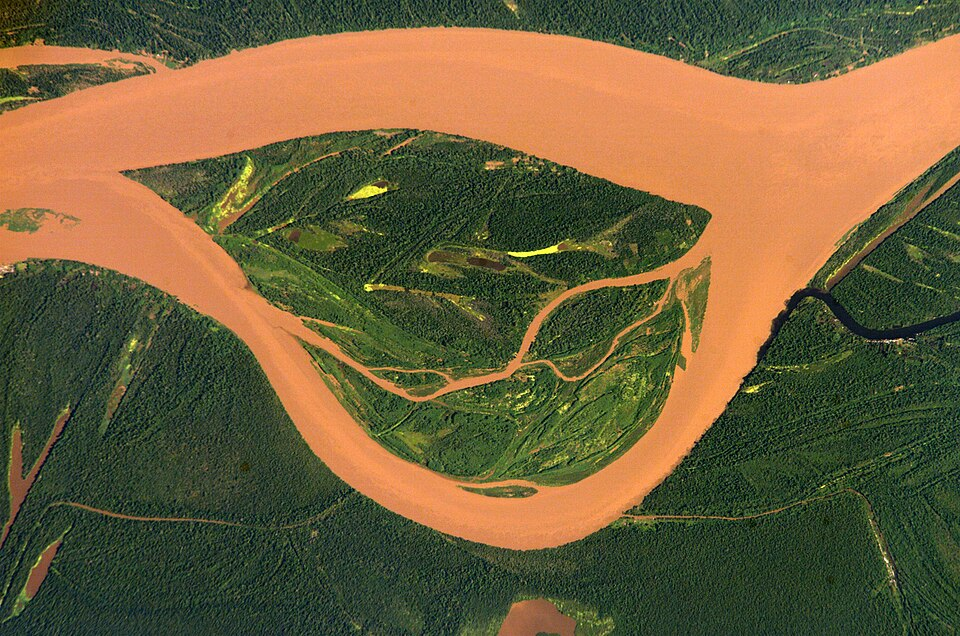
\includegraphics[width=0.6\linewidth]{images/book1/g4-amazon-iss.jpg}

{\small \omterm{def:g1:landscapes-around-us:water}{نهر} الأمازون، بنيًا من \omterm{def:g3:stones-pebbles-sand:sand}{الوحل}، يتلوى عبر الغابة المطيرة، كما يُرى من
محطة الفضاء الدولية. الصورة: NASA (ملك عام).}
% ledger: nasa:amazon-iss
\end{omfigure}

\omterm{def:g1:landscapes-around-us:water}{والبحيرات} أيضًا تحطم الأرقام. فأكبر \omterm{def:g1:landscapes-around-us:water}{بحيرة} على الأرض هي \omterm{def:g2:water-on-earth:ocean}{بحر} قزوين، بين
أوروبا وآسيا: إنها كبيرة إلى حد أنها تسمى بحرًا، لكن اليابسة تحيط بها من كل
جانب. وتغطي أكثر من
370\,000 كيلومتر مربع. وأعمق \omterm{def:g1:landscapes-around-us:water}{بحيرة} هي \omterm{def:g1:landscapes-around-us:water}{بحيرة} بايكال، في روسيا: ففي
بعض أماكنها يقع قاعها على عمق قرابة كيلومترين تحت سطحها.
% ledger: natgeo:caspian-baikal

\section{الصحاري والجليد العظيم}

نوعان من الأماكن يبرزان على \omterm{def:g4:world-physical-map:physical-map}{الخريطة الطبيعية} لأن شيئًا لا ينمو فيهما
تقريبًا: الصحاري الكبرى، حيث لا تمطر تقريبًا أبدًا، والجليد
العظيم.

الصحراء الكبرى، في شمال إفريقيا، أكبر صحراء حارة على الأرض. وتغطي نحو
ثمانية ملايين ونصف مليون كيلومتر مربع. وتغطي إفريقيا كلها نحو 30 مليون
كيلومتر مربع، فالصحراء الكبرى أكثر قليلًا من ربع \omterm{def:g3:continents-and-oceans:continent}{القارة}: أكثر من
$\frac{1}{4}$، لكنها أقل من
$\frac{1}{3}$.
% ledger: natgeo:sahara, data:etopo1

الجليد العظيم يغطي القارة القطبية الجنوبية، حول \omterm{def:g3:continents-and-oceans:poles}{القطب الجنوبي}، ويغطي معظم
غرينلاند، في أقصى شمال \omterm{def:g2:water-on-earth:ocean}{المحيط} الأطلسي. فهناك تراكم \omterm{def:g4:clouds-rain-snow:precipitation}{ثلج} آلاف السنين وتحول
إلى طبقة سميكة من الجليد. وعلى \omterm{def:g4:world-physical-map:physical-map}{الخريطة الطبيعية}، ألوانهما ألوان الأرض
المرتفعة، لأن سطح الجليد يعلو كثيرًا فوق \omterm{def:g4:world-physical-map:altitude}{مستوى سطح البحر}.

\section{الأعلى والأعمق}

\omterm{def:g4:world-physical-map:physical-map}{الخريطة الطبيعية} تبين شكل سطح الأرض، لكنها صغيرة إلى حد أنها تخفي
الأطراف القصوى. فلنضعها جنبًا إلى جنب، بمقياس رسم واحد.

\begin{omfigure}
\begin{tikzpicture}[x=1cm, y=0.32cm, font=\small]
  % sea level
  \fill[omHypsSeaA] (0,0) rectangle (9,-11.5);
  \fill[omHypsSeaD!80] (4.6,-11.5) -- (4.6,-11.0) -- (5.0,-10.98) -- (5.4,-11.0) -- (5.4,-11.5) -- cycle;
  \draw[black!60] (-0.2,0) -- (9.2,0);
  \node[anchor=west, font=\scriptsize] at (9.25,0) {\foreignlanguage{arabic}{مستوى سطح البحر \babelsublr{0\,m}}};
  % height scale
  \draw[black!60] (0,-11.5) -- (0,10);
  \foreach \h in {-10,-8,...,8} {
    \draw[black!60] (-0.1,\h) -- (0,\h);
    \node[anchor=east, font=\scriptsize] at (-0.12,\h) {\h\,km};
  }
  % ocean floor and trench
  \fill[brown!45] (0.05,-11.5) -- (0.05,-3.7) -- (3.2,-3.7) -- (4.4,-6) -- (4.9,-10.98) -- (5.1,-10.98)
    -- (5.6,-6) -- (6.4,-3.7) -- (9,-3.7) -- (9,-11.5) -- cycle;
  \node[font=\scriptsize, align=center] at (2.0,-5.3) {قاع المحيط\\\foreignlanguage{arabic}{على عمق نحو \babelsublr{3\,700\,m}}};
  \node[font=\scriptsize, anchor=west, align=left] at (5.6,-9.4) {أعمق نقطة\\غور تشالنجر\\\foreignlanguage{arabic}{نحو \babelsublr{11\,000\,m}}};
  % Everest
  \fill[black!35] (6.6,0) -- (7.6,8.85) -- (8.6,0) -- cycle;
  \fill[white, draw=black!45, line width=0.3pt] (7.35,6.6) -- (7.6,8.85) -- (7.85,6.6) -- (7.6,7.1) -- cycle;
  \node[font=\scriptsize, align=center, anchor=south] at (7.6,8.95) {\foreignlanguage{arabic}{جبل إفرست \babelsublr{8\,849\,m}}};
  % cirrus clouds band
  \draw[black!45, line width=0.6pt] (1.0,9.0) .. controls (1.6,9.5) and (2.2,9.1) .. (2.8,9.6);
  \draw[black!45, line width=0.6pt] (1.2,8.3) .. controls (1.8,8.8) and (2.4,8.4) .. (3.0,8.9);
  \node[font=\scriptsize, align=center] at (2.0,7.2) {سحب عالية\\\foreignlanguage{arabic}{(السمحاق)}};
  % a village
  \fill[black!60] (2.2,1.5) rectangle (2.45,1.75);
  \node[font=\scriptsize, anchor=west] at (2.5,1.6) {\foreignlanguage{arabic}{قرية جبلية \babelsublr{1\,500\,m}}};
\end{tikzpicture}

{\small من أعمق نقطة في \omterm{def:g2:water-on-earth:ocean}{المحيط} إلى أعلى قمة، بمقياس رسم واحد. فغور تشالنجر،
في \omterm{def:g2:water-on-earth:ocean}{المحيط} الهادئ، يقع تحت سطح \omterm{def:g2:water-on-earth:ocean}{البحر} على عمق أكبر من \omterm{def:g4:world-physical-map:altitude}{ارتفاع} \omterm{def:g1:landscapes-around-us:landform}{جبل} إفرست فوقه.
القيم: إفرست 8\,849\,m؛ غور تشالنجر قرابة 11\,000\,m؛ ومتوسط قاع \omterm{def:g2:water-on-earth:ocean}{المحيط}
نحو
3\,700\,m.}
\label{fig:g4:world-physical-map:extremes}
% ledger: tht:everest, usgs:trench-depth, nos:ocean-depth, wmo:cloud-levels
\end{omfigure}

\begin{example}[إفرست في الأعماق]\label{ex:g4:world-physical-map:everest-in-deep}
لو استطعنا أن نرفع \omterm{def:g1:landscapes-around-us:landform}{جبل} إفرست ونضعه في قاع غور تشالنجر، لبقيت قمته تحت
الماء: نحو 11\,000 متر من الغور، مقابل 8\,849 مترًا من \omterm{def:g1:landscapes-around-us:landform}{الجبل}. ولبقي فوقها
أكثر من كيلومترين من
\omterm{def:g2:water-on-earth:ocean}{البحر}.
% ledger: tht:everest, usgs:trench-depth
\end{example}

\section{تمارين}

\begin{exercise}[$\star$]\label{exo:g4:world-physical-map:1}
ما \omterm{def:g4:world-physical-map:altitude}{ارتفاع} مكان ما؟ ومن أي مستوى يُقاس؟
\end{exercise}

\begin{exercise}[$\star$]\label{exo:g4:world-physical-map:2}
مستعينًا \omterm{def:g2:drawing-to-map:legend}{بمفتاح} \omterm{def:g4:world-physical-map:physical-map}{الخريطة الطبيعية}، أعطِ \omterm{def:g4:world-physical-map:altitude}{ارتفاع} مكان
لونه: (أ) أخضر داكن؛ (ب) أصفر فاتح؛ (ج) أبيض تقريبًا.
\end{exercise}

\begin{exercise}[$\star$]\label{exo:g4:world-physical-map:3}
في أي \omterm{def:g3:continents-and-oceans:continent}{قارة} تقع: (أ) \omterm{def:g1:landscapes-around-us:landform}{جبال} الأنديز؛ (ب) \omterm{def:g1:landscapes-around-us:landform}{جبال} الهيمالايا؛ (ج) الصحراء الكبرى؛
(د) \omterm{def:g1:landscapes-around-us:landform}{جبال} روكي؟
\end{exercise}

\begin{exercise}[$\star$]\label{exo:g4:world-physical-map:4}
سمِّ أعلى \omterm{def:g1:landscapes-around-us:landform}{جبل} على الأرض، وأكبر \omterm{def:g1:landscapes-around-us:water}{بحيرة}، وأعمق \omterm{def:g1:landscapes-around-us:water}{بحيرة}.
\end{exercise}

\begin{exercise}[$\star$]\label{exo:g4:world-physical-map:5}
على \omterm{def:g4:world-physical-map:physical-map}{الخريطة الطبيعية}، \omterm{def:g2:water-on-earth:ocean}{البحر} قرب \omterm{def:g1:landscapes-around-us:water}{السواحل} أزرق فاتح ووسط المحيطات أزرق
داكن. ماذا يخبرك ذلك عن عمق \omterm{def:g2:water-on-earth:ocean}{البحر}؟
\end{exercise}

\begin{exercise}[$\star$]\label{exo:g4:world-physical-map:6}
لماذا لُوّنت القارة القطبية الجنوبية وغرينلاند كالأرض المرتفعة على \omterm{def:g4:world-physical-map:physical-map}{الخريطة
الطبيعية}؟
\end{exercise}

\begin{exercise}[$\star\star$]\label{exo:g4:world-physical-map:7}
رتّب من الأخفض إلى الأعلى: شاطئ؛ قرية على \omterm{def:g4:world-physical-map:altitude}{ارتفاع}
1\,500 متر؛ قمة \omterm{def:g1:landscapes-around-us:landform}{جبل} إفرست؛ قاع غور
تشالنجر؛ متوسط قاع \omterm{def:g2:water-on-earth:ocean}{المحيط}.
\end{exercise}

\begin{exercise}[$\star\star$]\label{exo:g4:world-physical-map:8}
لماذا لا نستطيع أن نقول يقينًا أيهما الأطول: النيل أم
الأمازون؟
\end{exercise}

\begin{exercise}[$\star\star$]\label{exo:g4:world-physical-map:9}
تغطي إفريقيا نحو 30 مليون كيلومتر مربع. فكم يساوي ربعها؟ وكم ثلثها؟
وتغطي الصحراء الكبرى نحو ثمانية ملايين ونصف مليون كيلومتر
مربع: فهل هي أكثر من ربع إفريقيا أم أقل؟ وأكثر من
ثلثها أم أقل؟
\end{exercise}

\begin{exercise}[$\star\star$]\label{exo:g4:world-physical-map:10}
يقوم كوخ جبلي على \omterm{def:g4:world-physical-map:altitude}{ارتفاع} 2\,500 متر، وتحته \omterm{def:g1:landscapes-around-us:water}{بحيرة} على \omterm{def:g4:world-physical-map:altitude}{ارتفاع} 1\,000
متر. بكم مترًا يعلو الكوخ؟ وما لون كل منهما على
\omterm{def:g4:world-physical-map:physical-map}{الخريطة الطبيعية}؟
\end{exercise}

\begin{exercise}[$\star\star\star$]\label{exo:g4:world-physical-map:11}
تطير طائرة على \omterm{def:g4:world-physical-map:altitude}{ارتفاع} 10 كيلومترات فوق \omterm{def:g4:world-physical-map:altitude}{مستوى سطح البحر}. فهل هي أعلى من \omterm{def:g1:landscapes-around-us:landform}{جبل}
إفرست؟ وبكم مترًا؟ ولو طارت فوق غور تشالنجر، فكم تكون بعيدة
عن قاع الغور (خذ 11\,000 متر عمقًا
للغور)؟
\end{exercise}
